
\pandocbounded{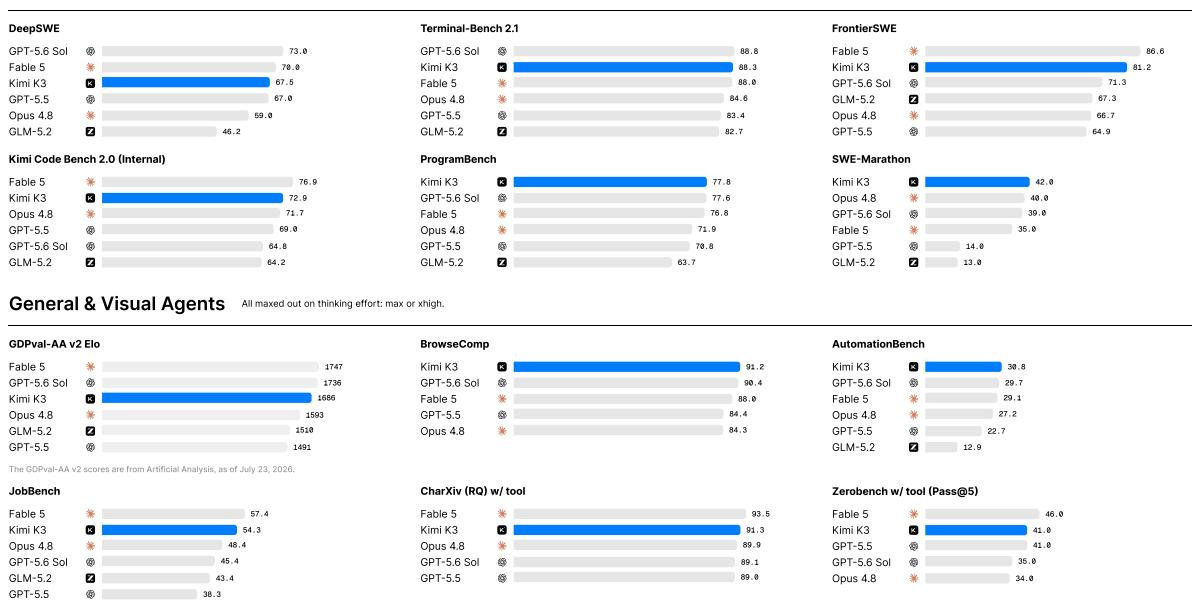
\includegraphics[keepaspectratio,alt={image}]{images/158fb68a657c2516b24b137b935b8d6f48a0d31f828efbcfd42cd83969a982d9.jpg}}

\begin{center}
{\LARGE KIMI K3：开放前沿智能\par}
\vspace{0.4em}
{\Large KIMI K3 技术报告\par}
\vspace{0.8em}
Kimi 团队
\end{center}

\section*{摘要}\label{abstract}

我们提出 Kimi K3，一个拥有 2.8 万亿参数的 Mixture-of-Experts 模型，激活参数为 1040 亿，具备原生视觉能力和 100 万 token 的上下文窗口。Kimi K3 基于 Kimi Delta Attention [63] 和 Attention Residuals [57]，这两项技术分别改善了沿序列长度和模型深度的信息流动。结合 Stable LatentMoE（每个 token 在 896 个路由专家中有效激活 16 个）以及经过优化的训练和数据方案，这些进展使整体扩展效率相比 Kimi K2 [58] 提升了约 2.5 倍。后训练方面，重点介绍了在通用、智能体和编程领域的强化学习，以及多个推理努力级别，从而实现了组合泛化和稳健的长期执行能力。在 2.8T 规模下，Kimi K3 得到了多个领域基础设施进步的支持：面向 KDA 的算法--系统协同设计、具有高效内存管理的完美均衡专家并行训练、支持持久化 rollout 和沙箱状态的百万 token 智能体强化学习，以及部署创新。

广泛的评估表明，Kimi K3 在长期编程、智能体、知识、推理和视觉任务上均达到了前沿水平。虽然其整体性能仍落后于最强大的闭源模型 Claude Fable 5 和 GPT-5.6 Sol，但 Kimi K3 始终优于我们评估套件中的其他开源和闭源模型。我们发布完整的 Kimi K3 模型权重，以促进未来研究，并加速前沿智能的更广泛部署和应用。

编程 AI 在思考努力上达到最大值：max 或 xhigh。

通用和视觉智能体 AI 在思考努力上达到最大值：max 或 xhigh。

注：Fable 5 的结果包含可能的回退。GPT-5.6 Sol 的结果包含可能的网络防护。

图 1: Kimi K3 主要结果。

\section{引言}\label{introduction}

在大语言模型 (LLM) 发展的相当长一段时期里，扩展意味着在部署前投入更多计算资源，通过训练更大的模型处理更多数据 [54, 45]。推理模型的兴起将测试时计算确立为第二维度上的扩展：OpenAI 的 o 系列扩展了强化学习和测试时推理 [84, 83]；Anthropic 的扩展思考模型分配自适应思考预算，并将推理与工具使用交织进行 [6, 7]；DeepSeek-R1 [40] 和 Kimi K1.5 [118] 表明，大规模强化学习能够从强大的预训练模型中激发出复杂的推理行为；Kimi K2.5 Agent Swarm [59] 进一步将测试时扩展从顺序推理推进到并行智能体协同。这些进步使测试时扩展成为前沿研究的核心焦点。然而，虽然开源模型生态在第二维度上进展迅速，但在第一维度上却进展缓慢：许多近期模型仍处于或略高于 1T 级参数区间 [145, 29, 135, 120]。随着日益复杂的推理和智能体强化学习方法被应用于规模相近的预训练基座，开源进展面临趋同的风险，而与最强闭源系统之间的差距则在不断扩大。凭借 Kimi K3，我们同时沿两条扩展轴向前沿推进：将预训练基座扩展到前所未有的 3T 级参数规模，同时在 100 万上下文长度上扩展强化学习、推理努力和长期交互。

我们提出 Kimi K3，一个原生多模态 Mixture-of-Experts 模型，总参数 2.8 万亿，激活参数 1040 亿，上下文窗口最长可达 100 万 token。其架构沿序列长度、网络深度和模型宽度三个维度扩展信息流。Kimi Delta Attention (KDA) [63] 提供高效的长序列混合，通过周期性插入的 Gated MLA 层保持全局交互。Attention Residuals (AttnRes) [57] 使每一层能够有选择地关注来自所有前置层的表示。Stable LatentMoE 将路由专家空间扩展到 896 个专家，每个 token 激活 16 个，同时通过归一化、SiTU-GLU 和 Quantile Balancing 在极端稀疏条件下稳定优化过程。这些架构进步结合优化的数据和训练方案，使整体扩展效率相比 Kimi K2 [58] 提升了约 2.5 倍。

我们将此预训练基座与专为 100 万上下文测试时扩展设计的后训练相结合。Kimi K3 在长期编程、通用智能体、通用推理和知识任务上进行了强化学习，每个任务跨越多个推理努力级别。训练环境包括可验证搜索与专业知识工作、软件工程与内核优化、带视觉回路工具使用的多模态推理、持久助手工作流、Web 开发以及自主执行任务。这些环境训练出一个推理、行动、观察、验证和适应的通用循环，通常涉及数百乃至数千次工具调用和数百万累积的上下文 token。领域和努力级别特化的策略通过多教师在线策略蒸馏 [75, 134, 29] 整合为一个统一模型。

实现这一目标需要基础设施随架构复杂度、模型规模和轨迹长度同步扩展。在面向 KDA 的系统协同设计方面，我们开发了融合内核、KDA Context Parallelism 和状态感知前缀缓存，使 KDA 在设备内、跨设备以及跨请求间均保持高效。针对 2.8T 参数的 MoE 预训练，MoonEP 通过静态计算形状和零拷贝通信实现完美均衡的专家执行，同时高效内存训练和多模态编码器优化在有限内存下维持利用率。针对百万 token 的智能体强化学习，我们的协同部署系统将部分 rollout、外部 KV-cache 保留、自适应限流和可恢复 microVM 沙箱相结合，以保持长生命周期的模型和环境状态。最后，特化内核以及缓存和预算感知的集群调度将这些创新转化为可预测的生产级服务。

最终模型确立了新的开放前沿。在涵盖长期编程、智能体、知识、推理和视觉任务的基准测试中，Kimi K3 整体上落后于最强的闭源系统——Claude Fable 5 和 GPT-5.6 Sol——并且始终领先于我们评估套件中的其他开源和闭源模型，如图 1 所示。

我们的贡献总结如下：

• 开放前沿的预训练。我们训练了一个 2.8T 参数的原生多模态 MoE 模型，激活参数 1040 亿，上下文窗口 100 万 token。KDA、AttnRes、Stable LatentMoE 以及优化的数据和训练方案共同使整体扩展效率相比 Kimi K2 提升了约 2.5 倍。

• 面向多努力级别测试时扩展的强化学习。我们在通用、智能体和编程领域以及多个推理努力级别上进行了强化学习，然后将由此获得的能力整合为一个统一模型。

• 面向数万亿参数、百万 token 智能的基础设施。我们引入了 KDA 系统协同设计；面向 2.8T 参数 MoE 预训练的 MoonEP 和高效内存基础设施；面向百万 token 智能体轨迹、支持可恢复沙箱的协同部署强化学习系统；以及更多基础设施创新。

• 一个开放前沿模型。我们发布完整的 Kimi K3 模型权重，使前沿智能可用于研究、部署和进一步创新。

\pandocbounded{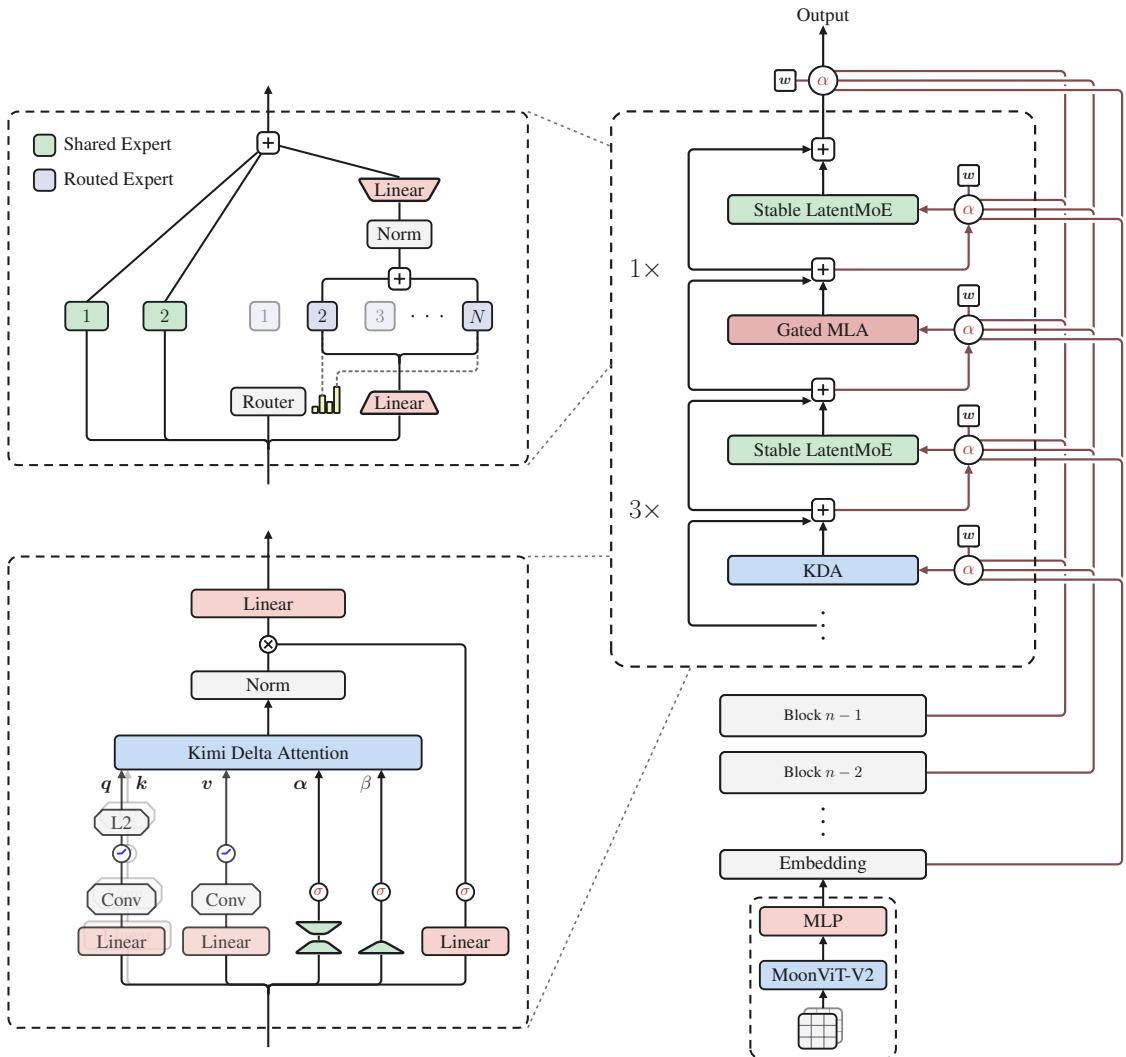
\includegraphics[keepaspectratio,alt={image}]{images/041827dc91ad4b391952d8a9464bb76f7ec75e33e3dd9098fd307db69b7dde9f.jpg}}

图 2: Kimi K3 架构，围绕 token 混合、通道混合和层混合组织，输入端具有原生视觉通路。每个 block 包含三个 Kimi Delta Attention (KDA) 层，后跟一个 Gated MLA 层，每个注意力层与一个 Stable LatentMoE 前馈网络配对。Attention Residuals (AttnRes) 使用可学习的伪查询 (w) 推导出对嵌入和前置 block 输出的注意力权重 (α)，实现跨深度的选择性信息流动。左上：Stable LatentMoE 模块，包含共享专家和路由专家。左下：KDA 模块。右下：原生视觉通路。
